\myframe{
  \ctr{Bem Vindos}
  \ctr{Estamos atrasados}
}

\myframe{
  \ctr{Estamos atrasados}
  \begin{itemize}
    \item A computação não é limitada por artigos;
    \item Internet, celulares, tablets, relógios\ldots;
    \item ``O matemático aplicado que tem que fazer a ponte'';
    \item Colaborações à distância.
  \end{itemize}
}

\myframe{
  \ctr{Todo mundo deveria aprender programação}
  \begin{itemize}
    \item ``I think everybody in this country should learn how to program a
      computer because it teaches you how to think.'' - Jobs, S.;
    \item Desenvolvimento de lógica e \emph{problem-solving skills};
    \item Facilitar algumas tarefas;
    \item Entender o mundo.
  \end{itemize}
}

\myframe{
  \ctr{Todo matemático deveria aprender programação}
  \begin{itemize}
    \item Melhorar a aula;
    \item Testar a teoria;
    \item Colaborar com outras pessoas.
  \end{itemize}
}

\myframe{
  \ctr{Terminal - Bash}
  \begin{itemize}
    \item Começamos aqui;
    \item Algumas coisas não se fazem com mouse;
    \item Grande quantidade de ferramentas;
    \item Todo computador (GNU/Linux) tem.
  \end{itemize}
}

\myframe{
  \ctr{Julia}
  \begin{itemize}
    \item Uma boa linguagem para pesquisadores das ciências exatas;
    \item Uma boa linguagem inicial;
    \item Almeja substituir o MatLab;
    \item Usa coisas boas de outras linguagens (C, Fortran, MatLab,
      Python,\ldots);
    \item Código aberto, ativamente desenvolvida.
  \end{itemize}
}

\myframe{
  \ctr{Git}
  \begin{itemize}
    \item Principal ferramenta livre de controle de versão;
    \item Colaboração;
    \item Qualquer arquivo de texto binário (\LaTeX, códigos);
    \item Versões diferentes (versão estável, de debug, conserto, nightly,
      etc.);
    \item Interfaces web e local para repositórios públicos e privados.
  \end{itemize}
}

\myframe{
  \begin{center}
    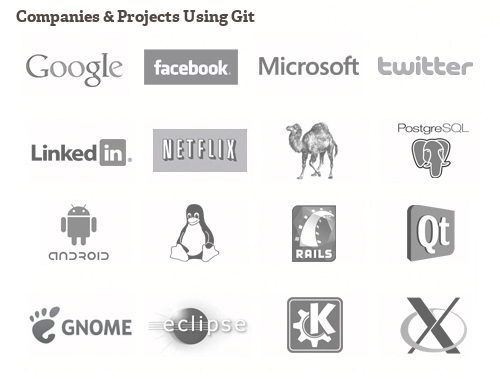
\includegraphics[height=0.9\textheight]{img/using-git.png}
  \end{center}
}
